\documentclass[aspectratio=43]{beamer}
\usetheme{Simple}

% Chinese support. Compile with LuaLaTeX or XeLaTeX.
\usepackage[UTF8,fontset=none]{ctex}
\setCJKmainfont[
  Path=/home/comp/zhanzhao/miniforge3/envs/latex/tinytex/texmf-dist/fonts/opentype/public/fandol/,
  Extension=.otf,
  BoldFont=FandolSong-Bold,
  ItalicFont=FandolKai-Regular
]{FandolSong-Regular}
\setCJKsansfont[
  Path=/home/comp/zhanzhao/miniforge3/envs/latex/tinytex/texmf-dist/fonts/opentype/public/fandol/,
  Extension=.otf,
  BoldFont=FandolHei-Bold
]{FandolHei-Regular}
\setCJKmonofont[
  Path=/home/comp/zhanzhao/miniforge3/envs/latex/tinytex/texmf-dist/fonts/opentype/public/fandol/,
  Extension=.otf
]{FandolFang-Regular}

\usepackage[]{graphicx}
\usepackage[]{amsmath}
\usepackage[]{amsfonts}
\usepackage[]{amssymb}
\usepackage[]{booktabs}
\usepackage[]{hyperref}
\usepackage[]{xcolor}
\usepackage[]{xurl}
\usepackage[]{multirow}
\setbeamertemplate{caption}[numbered]

\graphicspath{{Figures/}}

\newcommand{\tightitems}{\setlength{\itemsep}{2pt}\setlength{\parskip}{0pt}}
\newcommand{\AegisKV}{\textsc{AegisKV}}
\newcommand{\Critical}{\textsc{Critical}}
\newcommand{\NonCritical}{\textsc{Non-Critical}}

\def\meetingname{AegisKV Research Update}
\title{\AegisKV{}：面向 Agentic LLM Serving 的 Workflow-Aware KV 备份}
\subtitle{问题建模、实验设计与当前结果}
\author[Z Zhao]{Zhan Zhao}
\institute[HKBU]{Hong Kong Baptist University}
\date[\today]{\meetingname\\\today}

\hfuzz=100pt
\hbadness=10000
\vfuzz=100pt
\vbadness=10000
\emergencystretch=\maxdimen

\begin{document}

\begin{frame}[plain]
  \titlepage
\end{frame}

\begin{frame}{Outline}
  \tableofcontents
\end{frame}

%------------------------------------------------------------
\section{问题与建模}
%------------------------------------------------------------

\begin{frame}{问题：KV 丢失影响的是 Workflow WCT}
  \small
  \begin{itemize}
    \tightitems
    \item Agentic serving 中，一个 workflow 由多个 agentic 请求组成，请求可能分布在不同 GPU / node 上。
    \item 故障发生时，单个 request 的恢复时间并不能直接代表最终目标；真正目标是 workflow completion time (WCT)。
  \end{itemize}

  \vspace{0.3cm}
  \begin{block}{AegisKV 的核心问题}
    在有限 GPU HBM 中，如何决定每个 GPU 上多少空间用于正常 inference，多少空间用于 GPU-resident backup KV，并只为高价值 Agent 提供 GPUReplica。
  \end{block}
\end{frame}

\begin{frame}{Agent 类型：只为 Critical Agent 做 GPUReplica}
  \small
  \begin{columns}[T,onlytextwidth]
    \begin{column}{0.48\textwidth}
      \begin{block}{Critical Agent}
        \begin{itemize}
          \tightitems
          \item 对 WCT 或恢复路径影响大
          \item KV segment 可进入 GPUReplica 候选集合
          \item 用于计算 backup coverage 和 restore benefit
        \end{itemize}
      \end{block}
    \end{column}
    \begin{column}{0.48\textwidth}
      \begin{block}{Non-Critical Agent}
        \begin{itemize}
          \tightitems
          \item 仍正常执行并影响排队和 WCT
          \item 不占用 GPUReplica budget
          \item 只走普通 prefix cache、HostBackup 或 recompute
        \end{itemize}
      \end{block}
    \end{column}
  \end{columns}

  \vspace{0.25cm}
  \footnotesize
  本文不固定 workflow 拓扑。workflow 可以有不同 stage、fan-out、fan-in；只要求每个 agentic 请求携带 \texttt{critical\_agent} 标签。
\end{frame}

\begin{frame}{每个 GPU 的 Backup / Inference 划分}
  \small
  对单个 GPU，设可用于 serving 控制的 HBM 总预算为 $M$，用 $\alpha_t \in [0,1]$ 表示分给 Backup partition 的比例：

  \vspace{0.2cm}
  \begin{align*}
    M_{\mathrm{Backup}}(t) &= \alpha_t M \\
    M_{\mathrm{Inference}}(t) &= (1 - \alpha_t)M
  \end{align*}

  \begin{itemize}
    \tightitems
    \item $M_{\mathrm{Backup}}(t)$：GPU-resident backup KV，例如 peer replica 或 ACKed safe frontier。
    \item $M_{\mathrm{Inference}}(t)$：active KV、prefix cache 和 continuous batching admission。
    \item 多 GPU 时，决策为 $\boldsymbol{\alpha}_t=(\alpha_{1,t},\ldots,\alpha_{G,t})$。
  \end{itemize}
\end{frame}

\begin{frame}{Workflow-Level Reward}
  \small
  令 $\mathcal{W}_t$ 表示当前 decision window 中完成或被 failure replay 覆盖的 workflow 集合：

  \vspace{-0.1cm}
  \begin{align*}
    r_t
    =
    &\mathbb{E}_{w \sim \mathcal{W}_t}
    \left[
      \mathbf{1}\left[
        \operatorname{WCT}(w) \le \tau_{\mathrm{SLO}}
      \right]
    \right] \\
    &-
    \lambda
    \max\left(
      0,\,
      \operatorname{P99}_{\mathrm{WCT}}(t)-\tau_{\mathrm{SLO}}
    \right)
    -
    \eta\sum_{g=1}^{G}O_{g,t}
  \end{align*}

  \footnotesize
  这个 reward 只定义一次，并回传给整组 $\boldsymbol{\alpha}_t$。它不尝试把一个 workflow 的 WCT 强行拆成每个 node 的局部 reward。
\end{frame}

\begin{frame}{GPUReplica Placement：只看 Critical Segment}
  \small
  令 $\mathcal{N}_t$ 表示当前 window 中所有可见 KV segment。Critical Agent segment 集合为：

  \vspace{-0.1cm}
  \[
    \mathcal{C}_t =
    \{n \in \mathcal{N}_t \mid \operatorname{critical}(n)=1\}
  \]

  \[
    x_{n,t}=0,\quad
    \forall n \in \mathcal{N}_t \setminus \mathcal{C}_t
  \]

  \[
    \sum_{n \in \mathcal{C}_{g,t}}
    x_{n,g,t}\operatorname{size}(n)
    \le
    \alpha_{g,t}M_g(t)
  \]

  \footnotesize
  Non-Critical segment 的 GPUReplica utility 设为 0。它们仍可通过普通 prefix cache、HostBackup 或 recompute 恢复。
\end{frame}

\begin{frame}{Segment Utility 与 Restore Lower Envelope}
  \small
  Critical segment 的基础价值：

  \vspace{-0.1cm}
  \[
    V(n,t)
    =
    I_{\mathrm{wf}}(n,t)
    C_{\mathrm{redo}}(n,t)
    P_{\mathrm{fail}}(\operatorname{owner}(n),t)
    P_{\mathrm{reuse}}(n,t)
  \]

  \[
    U(n,t)=
    V(n,t)
    -C_{\mathrm{backup}}(n,t)
    -C_{\mathrm{restore}}(n,t)
    -C_{\mathrm{dup}}(n,t)
  \]

  \begin{block}{Failure 后不默认 restore}
    \[
      \begin{aligned}
        A_t^{\mathrm{restore}}(n)
        &=
        \arg\min_{a \in \mathcal{A}_{\mathrm{restore}}} C_a(n,t) \\
        \mathcal{A}_{\mathrm{restore}}
        &=
        \{\mathrm{gpu},\mathrm{host},\mathrm{cache},\mathrm{recompute}\}
      \end{aligned}
    \]
  \end{block}
\end{frame}

%------------------------------------------------------------
\section{实验设计}
%------------------------------------------------------------

\begin{frame}{系统位置}
  \begin{figure}
    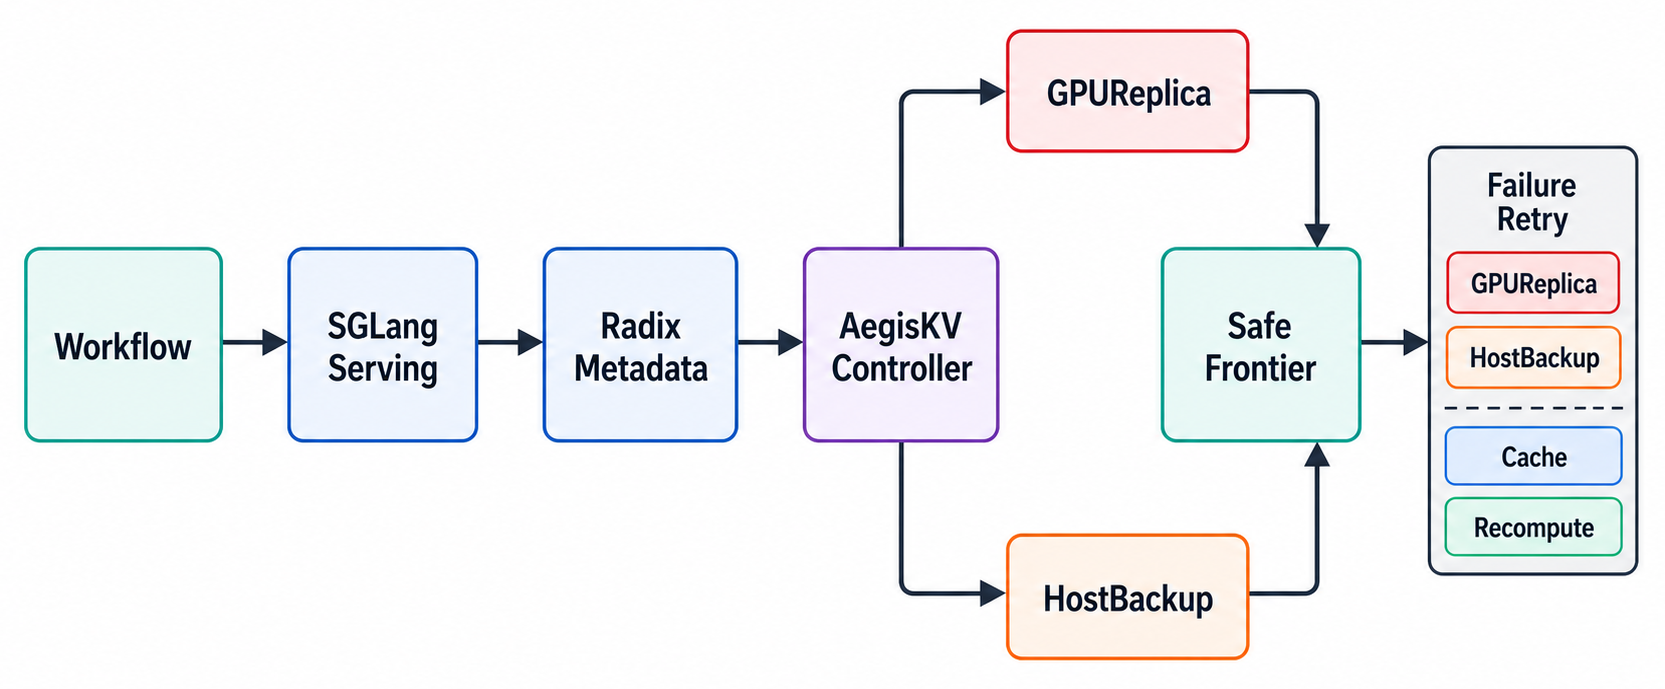
\includegraphics[width=0.98\textwidth]{fig_system_overview_generated_v2_tight.png}
  \end{figure}
  \vspace{-0.2cm}
  \footnotesize
  \AegisKV{} 在 SGLSim/SGLang serving path 中记录 backup frontier、GPUReplica coverage、retry route 和恢复动作。
\end{frame}

\begin{frame}{SGLSim 实现路径}
  \small
  \begin{columns}[T,onlytextwidth]
    \begin{column}{0.54\textwidth}
      \begin{block}{请求侧 metadata}
        \footnotesize
        \begin{itemize}
          \tightitems
          \item \texttt{workflow\_id / stage\_id}
          \item \texttt{critical\_agent / decode\_dominant}
          \item \texttt{backup\_kv / aegis\_policy}
          \item \texttt{retry\_dp\_rank / force\_dp\_rank}
        \end{itemize}
      \end{block}
    \end{column}
    \begin{column}{0.42\textwidth}
      \begin{block}{Runtime hooks}
        \footnotesize
        \begin{itemize}
          \tightitems
          \item \texttt{scheduler.py}
          \item \texttt{types.py}
          \item \texttt{alpha\_policy.py}
          \item \texttt{recovery\_model.py}
        \end{itemize}
      \end{block}
    \end{column}
  \end{columns}

  \vspace{0.2cm}
  \footnotesize
  Client 将 workflow/stage/criticality 写入每个 HTTP request 的 \texttt{simulation} 字段；scheduler 根据 Critical pressure 和 failure rate 选择 $\alpha$，并记录 frontier、GPUReplica coverage、failure replay 和 restore/recompute path。
\end{frame}

\begin{frame}{Workload 构造与 Failure Replay}
  \small
  \begin{columns}[T,onlytextwidth]
    \begin{column}{0.48\textwidth}
      \textbf{1-3-1-3-1 workflow}
      \begin{itemize}
        \tightitems
        \item 每个 workflow 是 9 个 agent session
        \item 单点 stage 的 agent 均为 Critical
        \item 两个 3-way stage 各有一个 long-decode Critical agent
        \item 其他 fan-out agent 为 Non-Critical
      \end{itemize}
    \end{column}
    \begin{column}{0.48\textwidth}
      \textbf{Failure replay}
      \begin{itemize}
        \tightitems
        \item 正常请求完成后记录 frontier
        \item 对 source DP rank 注入 failure
        \item retry 强制路由到健康 rank
        \item 只对 Critical session 做 replay
      \end{itemize}
    \end{column}
  \end{columns}

  \vspace{0.2cm}
  \begin{block}{可测信号}
    \footnotesize
    \texttt{request\_details.csv} 记录 \texttt{workflow\_id}、\texttt{stage\_id}、\texttt{decode\_dominant}、\texttt{critical\_agent}、\texttt{aegis\_gpu\_budget\_fraction}、restore action、recompute tokens 和 WCT 所需 latency。
  \end{block}

  \vspace{0.04cm}
  \scriptsize
  Generator audit: 27 requests / 9 slots，15 Critical / 12 Non-Critical；failure audit: 540 Critical-only soft retries，Non-Critical retry=0。
\end{frame}

%------------------------------------------------------------
\section{已有结果}
%------------------------------------------------------------

\begin{frame}{当前证据状态}
  \footnotesize
  \begin{columns}[T,onlytextwidth]
    \begin{column}{0.48\textwidth}
      \begin{block}{图表资产}
        \begin{itemize}
          \tightitems
          \item 25 张图已有 PNG 和 manifest
          \item Fig. 1/1b/1c 已更新为 fan-out stage-barrier trace-derived 动机图
          \item Fig. 3b/3c 已通过 MDP policy 与 runtime selector 一致性审计
          \item Fig. 3d 已加入 staged alpha risk tradeoff
          \item 24 张定量图已全部插入 Beamer
          \item Beamer 不插入详细机制流程图
        \end{itemize}
      \end{block}
    \end{column}
    \begin{column}{0.48\textwidth}
      \begin{block}{证据边界}
        \begin{itemize}
          \tightitems
          \item HPCA hybrid gate: 25/25 ready
          \item Goal audit: 17/17 pass，0 partial，0 blocked
          \item strict-final quantitative: Fig. 10b only
          \item alpha raw trace replay: 270/270 matched
          \item P0 restore: 693 rows，copy=693，bridge=693，schema missing=0
          \item P0 live-copy events: required 693，measured 693，H2D 375，P2P 318
          \item P2P remote plan: p2p\_live\_copy\_complete，rows 318
          \item SGLang matrix: accepted 6/6，wait-complete 3/3
          \item r2/r3 Slurm: 4 jobs complete，poll 00:43；complete 后 sync/audit
        \end{itemize}
      \end{block}
    \end{column}
  \end{columns}
\end{frame}

\begin{frame}{结果 1：同样大小 KV Loss，WCT 影响不同}
  \begin{figure}
    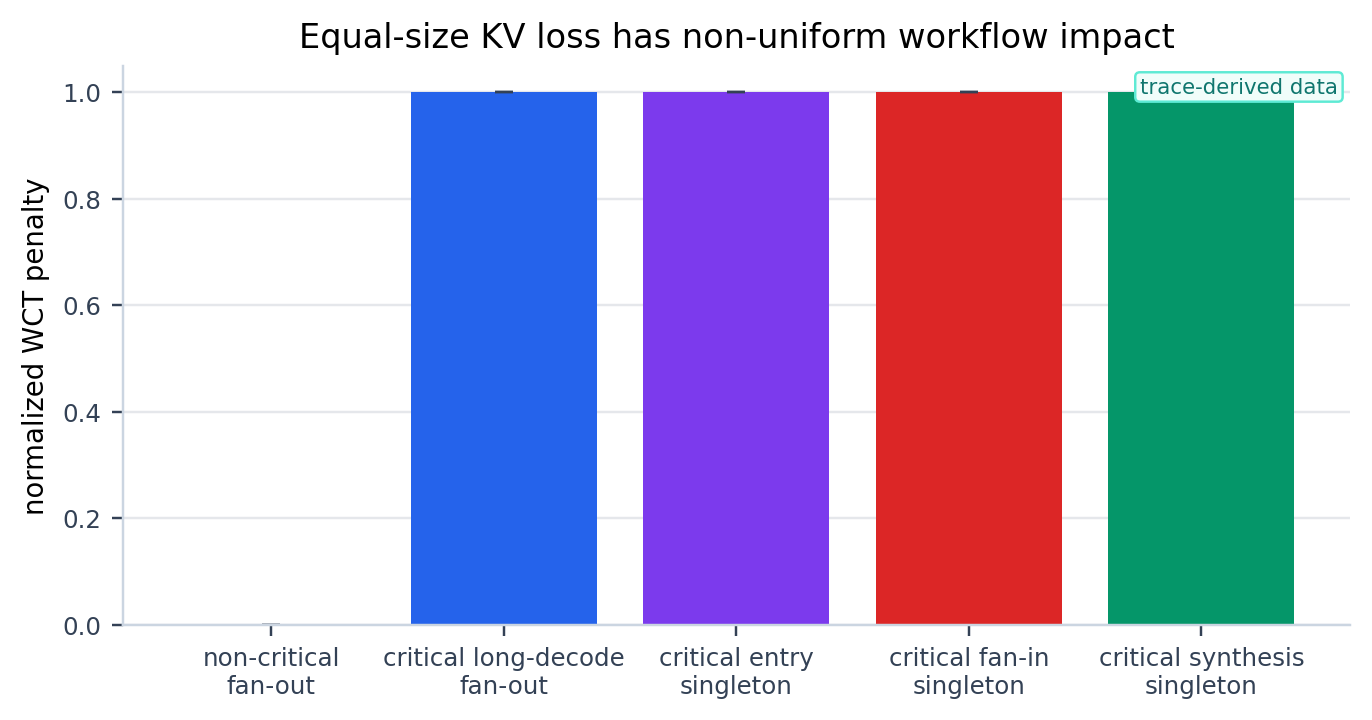
\includegraphics[width=0.88\textwidth]{fig_motivation_equal_size_loss.png}
  \end{figure}
  \vspace{-0.2cm}
  \footnotesize
  Fig. 1 来自 fan-out stage-barrier SGLSim trace：相同 token 数的 KV loss，在 Critical session 上暴露为 WCT penalty，在 Non-Critical fan-out 上被 slack 吸收。
\end{frame}

\begin{frame}{动机 2：Long-Decode Agent 是 Fan-out 瓶颈}
  \begin{figure}
    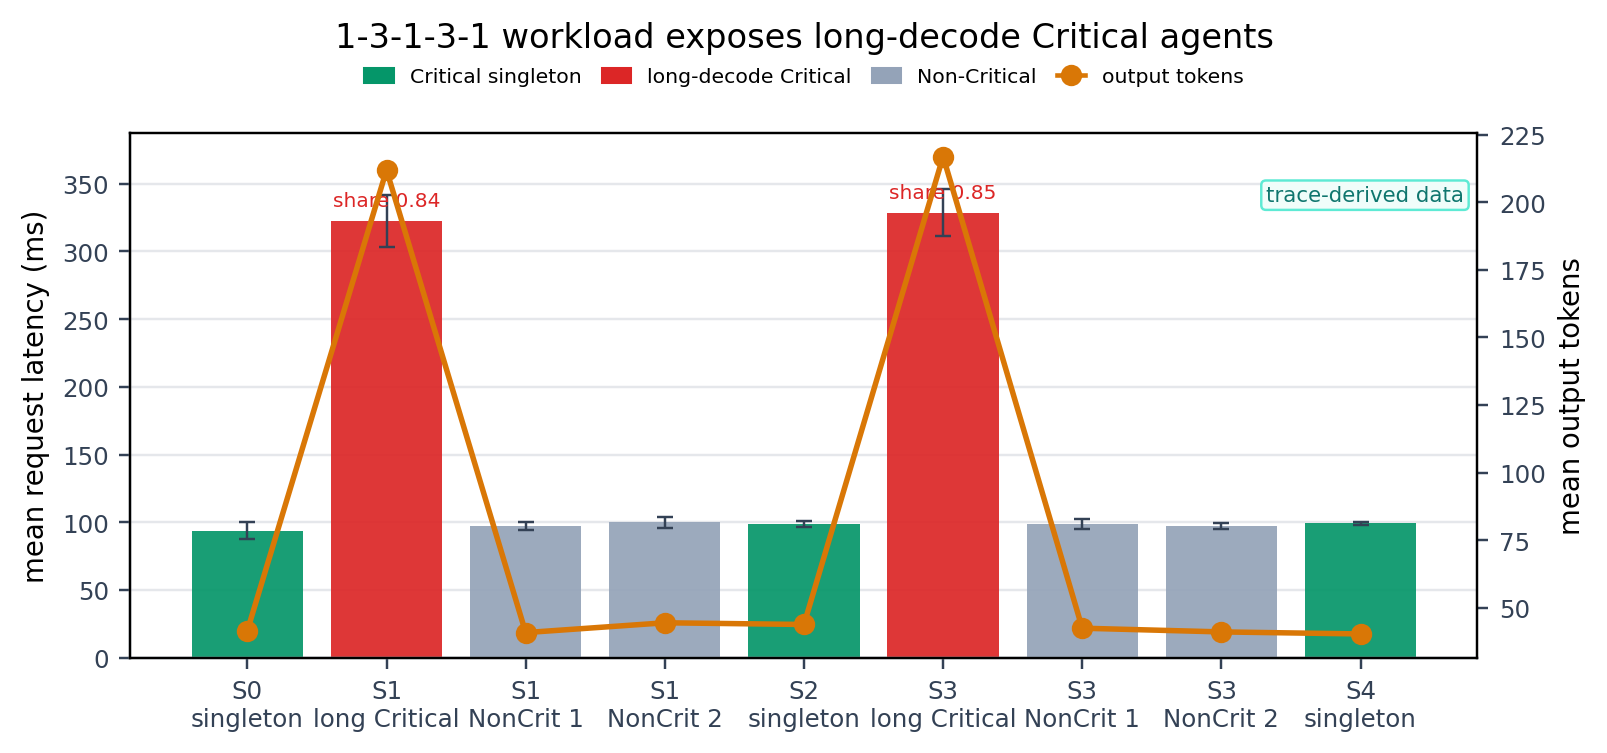
\includegraphics[width=0.92\textwidth]{fig_critical_agent_profile.png}
  \end{figure}
  \vspace{-0.2cm}
  \footnotesize
  1-3-1-3-1 workflow 中，两个 3-way fan-out stage 的 local agent 0 具有约 5 倍输出 token 和约 3 倍 latency，因此成为该 stage 的 Critical Agent；216 条 raw request trace 逐行匹配 singleton Critical / fan-out local-0 Critical / 其他 fan-out Non-Critical。
\end{frame}

\begin{frame}{动机 3：Critical Agent 应优先 Backup}
  \begin{figure}
    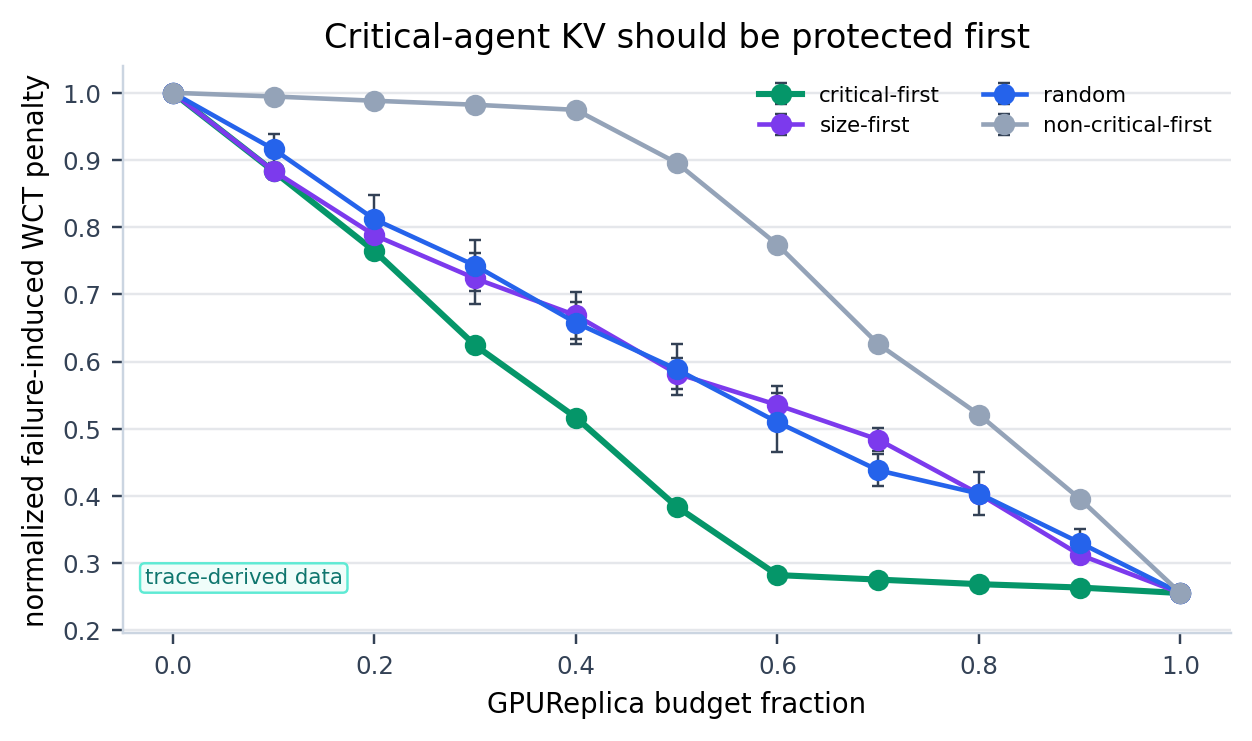
\includegraphics[width=0.90\textwidth]{fig_critical_backup_priority.png}
  \end{figure}
  \vspace{-0.2cm}
  \footnotesize
  1-3-1-3-1 workflow 中，单点 stage 和 fan-out 中长 decode agent 决定 WCT tail；同等 GPUReplica budget 下，Critical-first placement 的 WCT 收益最大。
\end{frame}

\begin{frame}{动机 4：$\alpha$ 取决于 Workload 与 Failure Risk}
  \begin{figure}
    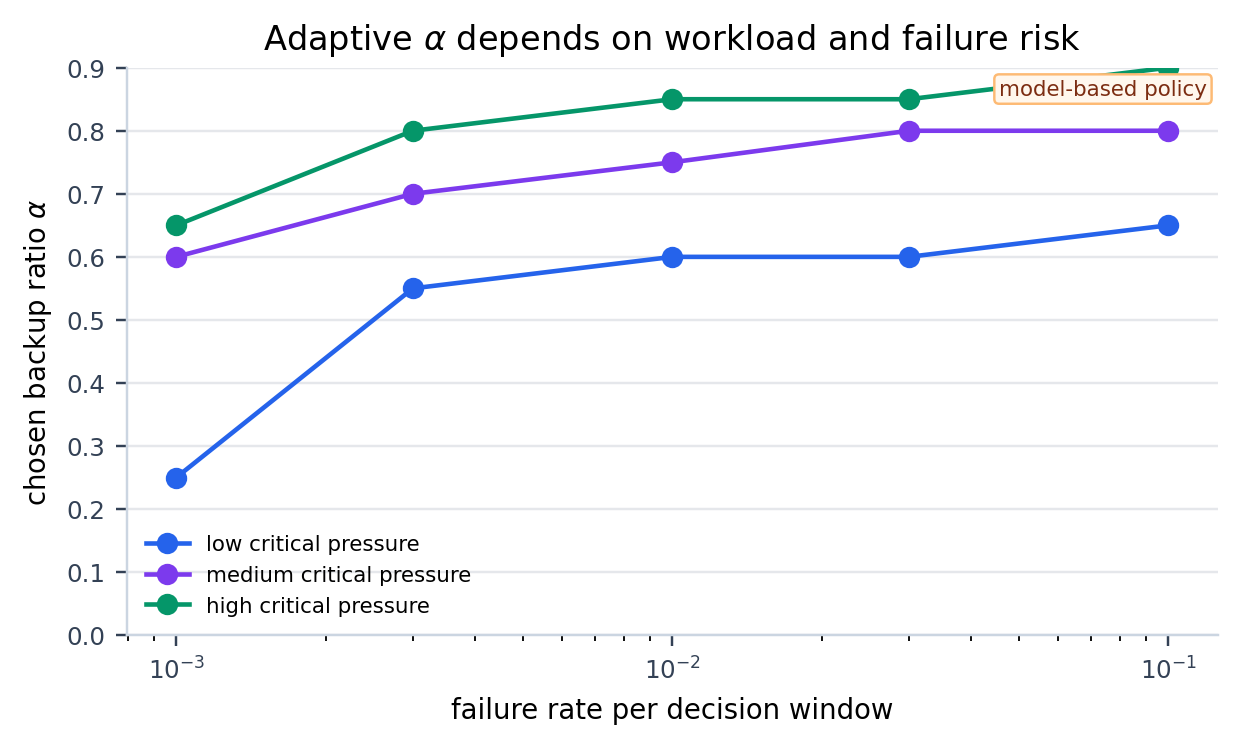
\includegraphics[width=0.88\textwidth]{fig_alpha_workload_failure_policy.png}
  \end{figure}
  \vspace{-0.2cm}
  \footnotesize
  Backup HBM ratio $\alpha$ 不是静态常数；Critical pressure 越高、failure risk 越高，在线 controller 应分配更多 HBM 给 GPUReplica。
\end{frame}

\begin{frame}{动机 5：Online $\alpha$ 随 Pressure 与 Risk 调整}
  \begin{figure}
    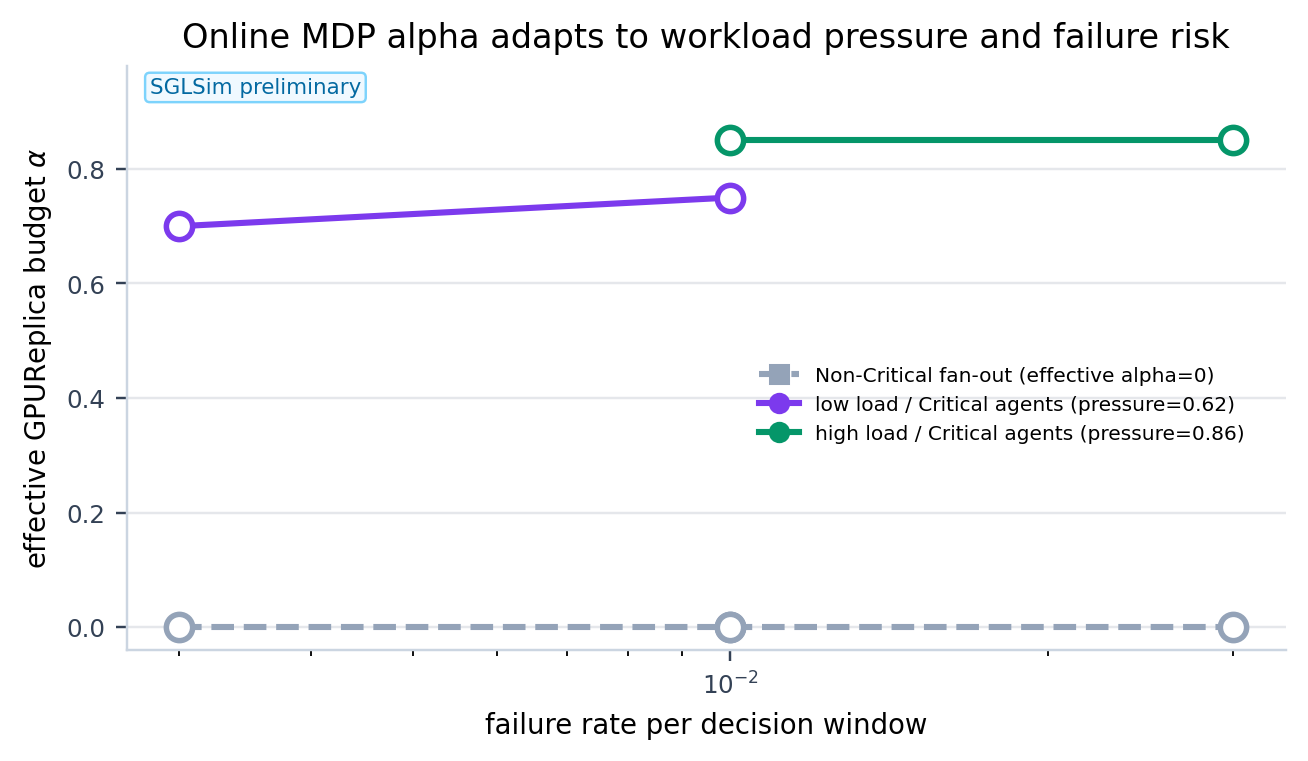
\includegraphics[width=0.88\textwidth]{fig_online_alpha_adaptation.png}
  \end{figure}
  \vspace{-0.2cm}
  \footnotesize
  1-3-1-3-1 online sweep 中，request stats 记录了 \texttt{policy\_table} source、workload pressure、failure-rate state 和实际选出的 $\alpha$；审计逐行重放 270 条 raw trace，确认 runtime selector 与 policy table 输出一致，Non-Critical effective GPUReplica budget 为 0。
\end{frame}

\begin{frame}{动机 6：Failure Risk 改变最优 $\alpha$}
  \begin{figure}
    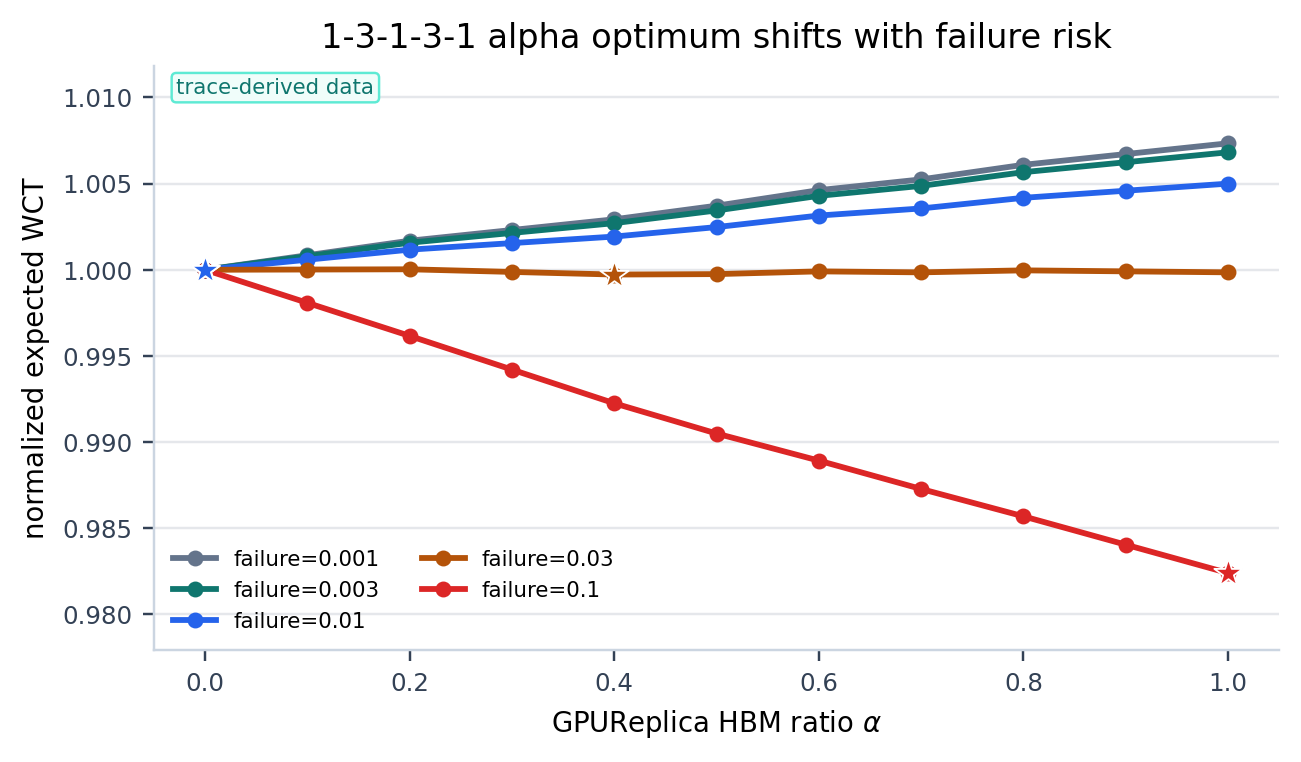
\includegraphics[width=0.88\textwidth]{fig_staged_alpha_risk_tradeoff.png}
  \end{figure}
  \vspace{-0.2cm}
  \footnotesize
  同一个 1-3-1-3-1 stage-barrier trace 上，低 failure risk 时可见 backup cost 主导，较小 $\alpha$ 更优；高 failure risk 时 recovery saving 主导，较大 $\alpha$ 降低 expected WCT。
\end{frame}

\begin{frame}{结果 2：Restore Boundary 与 GPUReplica Budget}
  \begin{columns}[T,onlytextwidth]
    \begin{column}{0.50\textwidth}
      \begin{figure}
        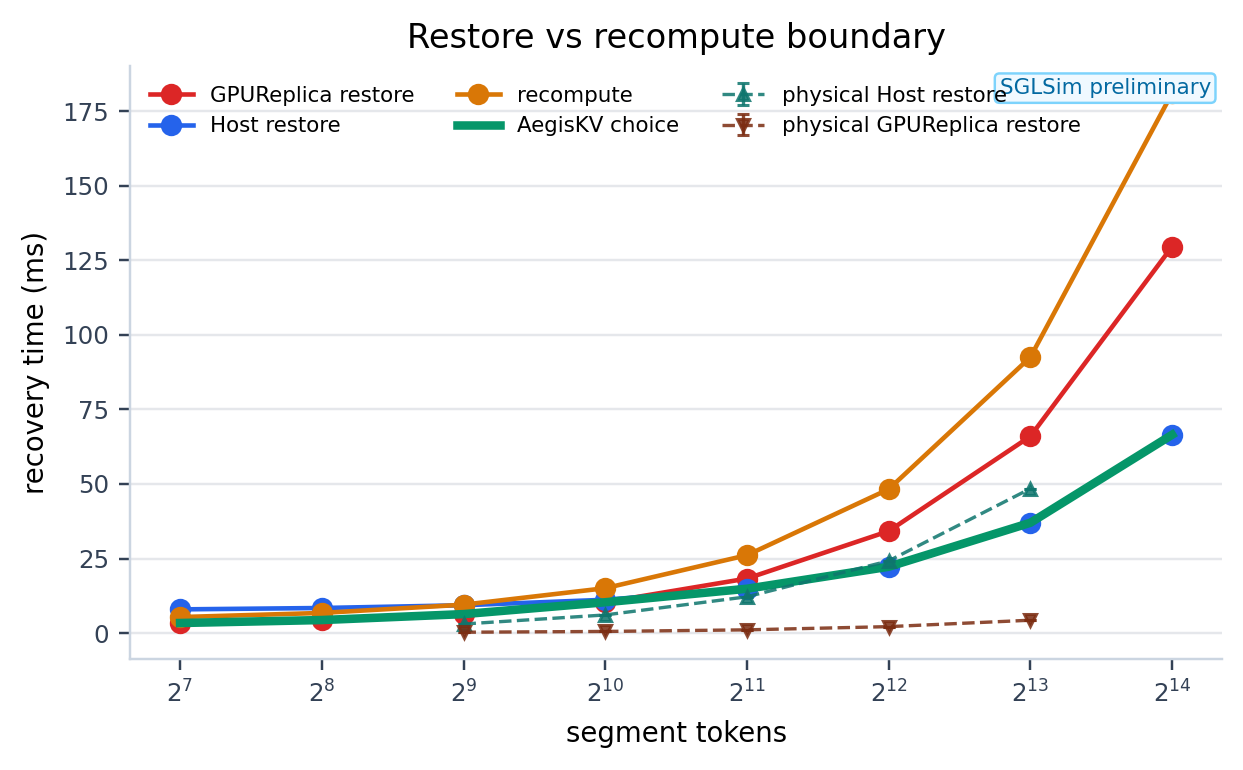
\includegraphics[width=\textwidth]{fig_restore_recompute_boundary.png}
      \end{figure}
      \vspace{-0.3cm}
      \centering\scriptsize Restore / recompute lower envelope
    \end{column}
    \begin{column}{0.50\textwidth}
      \begin{figure}
        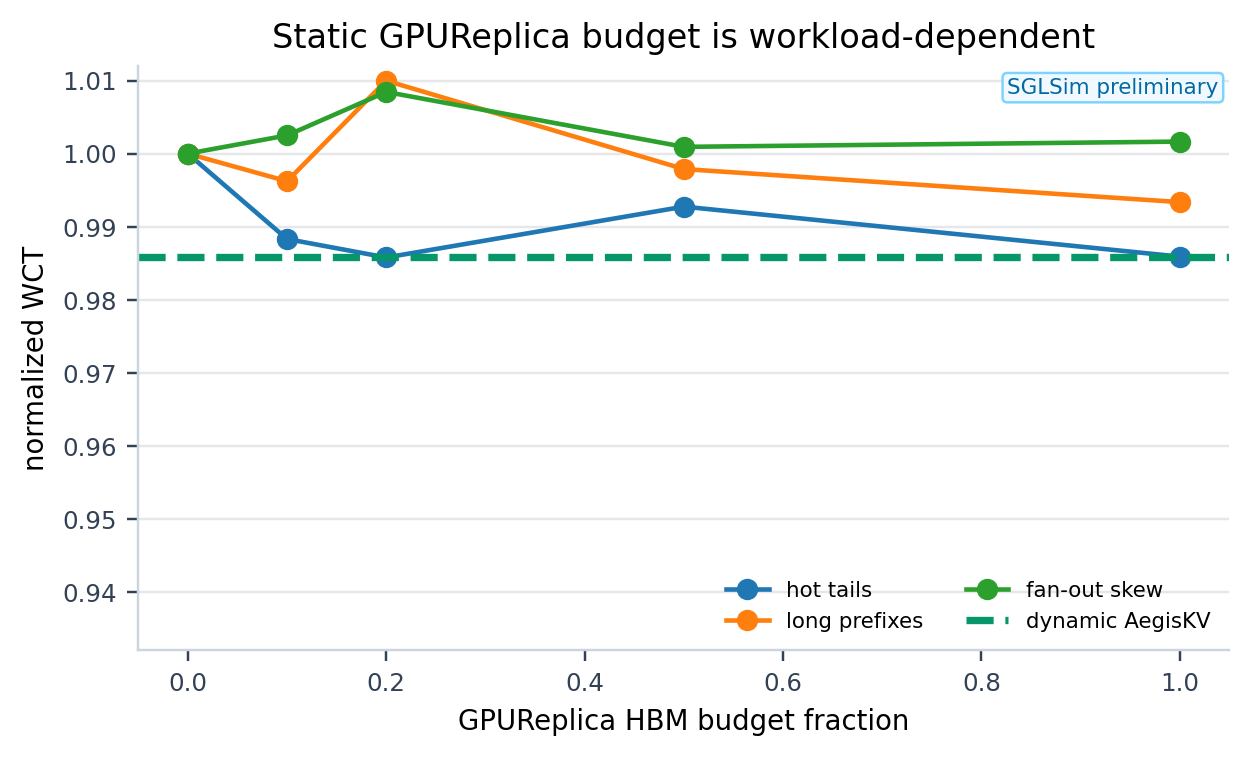
\includegraphics[width=\textwidth]{fig_static_gpu_replica_budget_gap.png}
      \end{figure}
      \vspace{-0.3cm}
      \centering\scriptsize Static GPUReplica budget gap
    \end{column}
  \end{columns}

  \vspace{0.1cm}
  \footnotesize
  Restore/recompute 的最优路径由 token 数和物理 copy cost 决定；固定 GPUReplica budget 在不同 workload regime 下不是全局最优。
\end{frame}

\begin{frame}{结果 3：Total WCT 与 Failure-Exposed Cost}
  \begin{columns}[T,onlytextwidth]
    \begin{column}{0.50\textwidth}
      \begin{figure}
        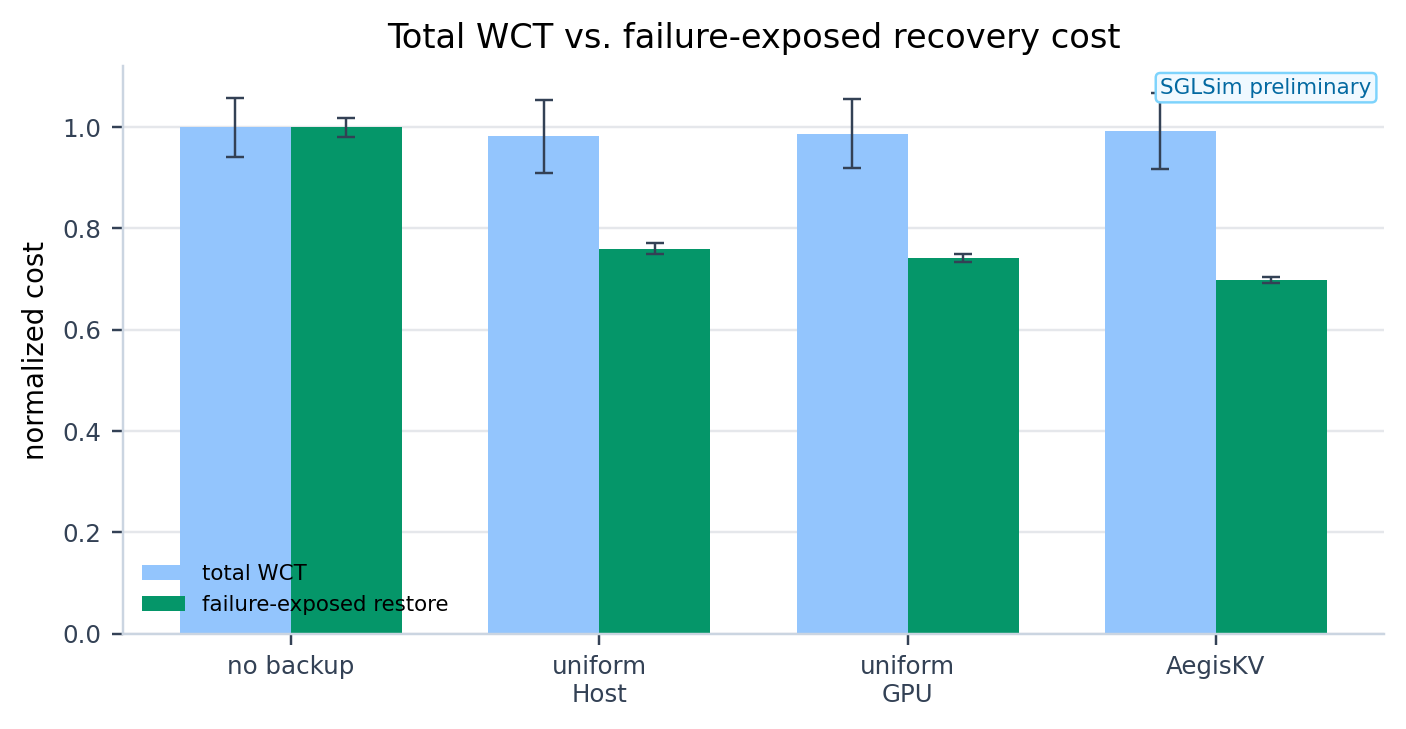
\includegraphics[width=\textwidth]{fig_overall_wct.png}
      \end{figure}
      \vspace{-0.3cm}
      \centering\scriptsize Total WCT and exposed restore cost
    \end{column}
    \begin{column}{0.50\textwidth}
      \begin{figure}
        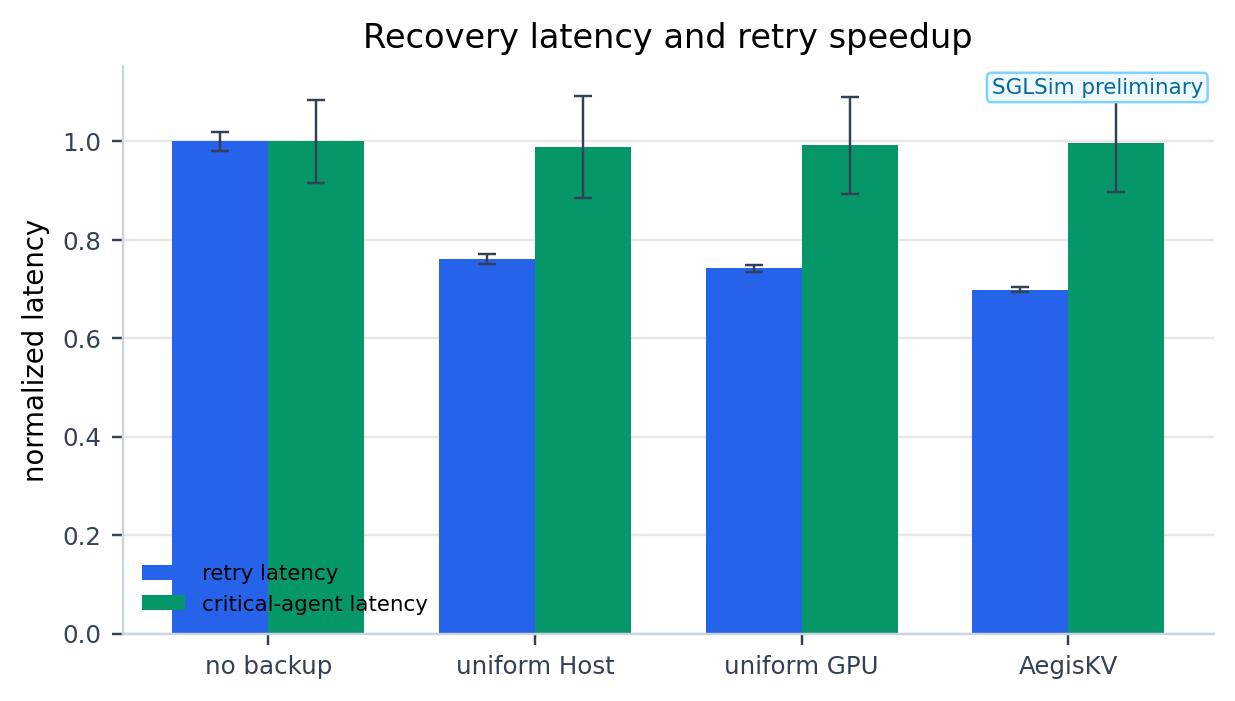
\includegraphics[width=\textwidth]{fig_recovery_latency.png}
      \end{figure}
      \vspace{-0.3cm}
      \centering\scriptsize Recovery latency sweep
    \end{column}
  \end{columns}

  \vspace{0.1cm}
  \footnotesize
  当前为 SGLSim preliminary / hybrid-ready 证据。Total WCT 被正常 serving 时间稀释；failure-exposed restore cost 和 retry latency 更直接体现 AegisKV 的恢复收益。
\end{frame}

\begin{frame}{结果 4：Restore Path 与 Shared Prefix}
  \begin{columns}[T,onlytextwidth]
    \begin{column}{0.50\textwidth}
      \begin{figure}
        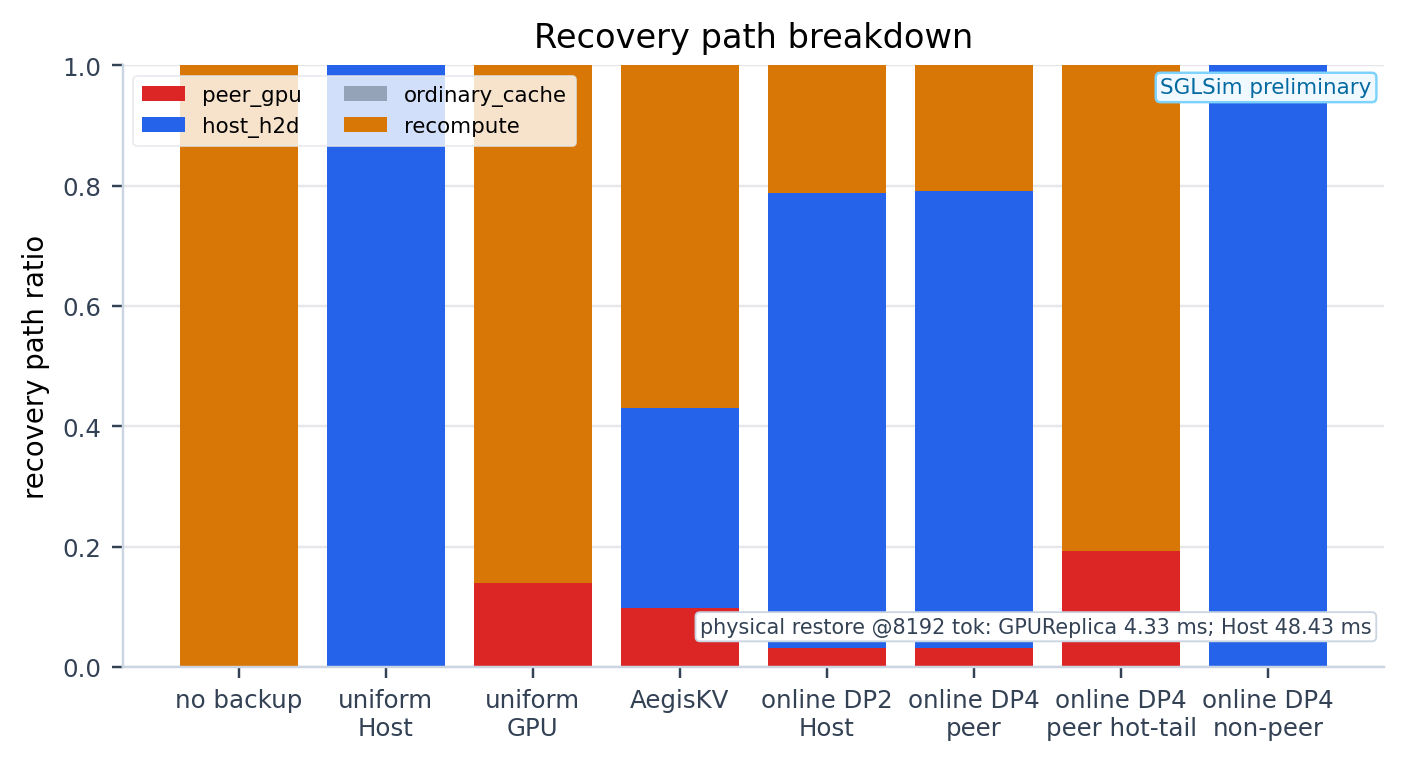
\includegraphics[width=\textwidth]{fig_recovery_path_breakdown.png}
      \end{figure}
      \vspace{-0.3cm}
      \centering\scriptsize Host / GPUReplica / cache / recompute
    \end{column}
    \begin{column}{0.50\textwidth}
      \begin{figure}
        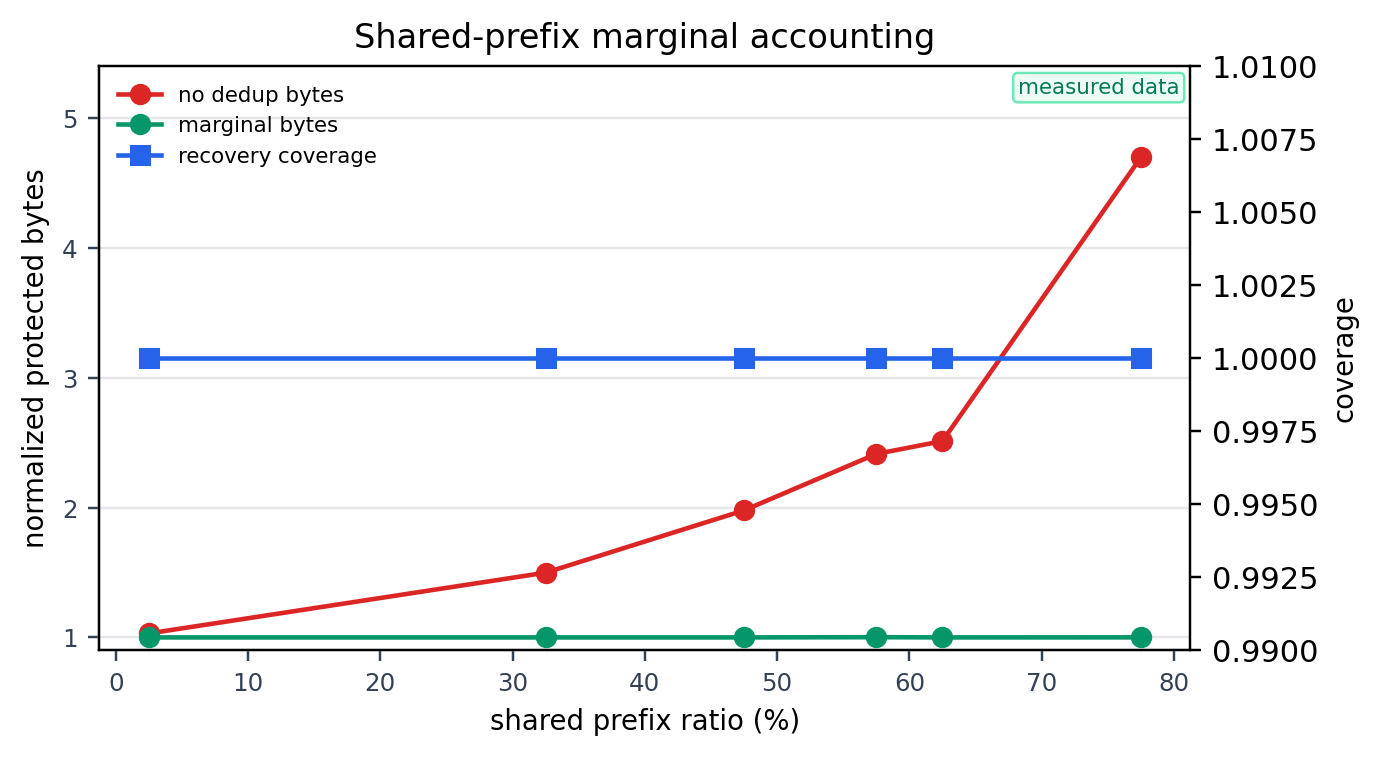
\includegraphics[width=\textwidth]{fig_shared_prefix_marginal.png}
      \end{figure}
      \vspace{-0.3cm}
      \centering\scriptsize Marginal SafeCover accounting
    \end{column}
  \end{columns}

  \vspace{0.1cm}
  \footnotesize
  Fig. 10b 是 strict-final-ready：shared prefix 不能重复计算收益，marginal accounting 能减少重复保护。
\end{frame}

\begin{frame}{结果 5：Normal-Path Overhead 与 Calibration}
  \begin{columns}[T,onlytextwidth]
    \begin{column}{0.52\textwidth}
      \begin{figure}
        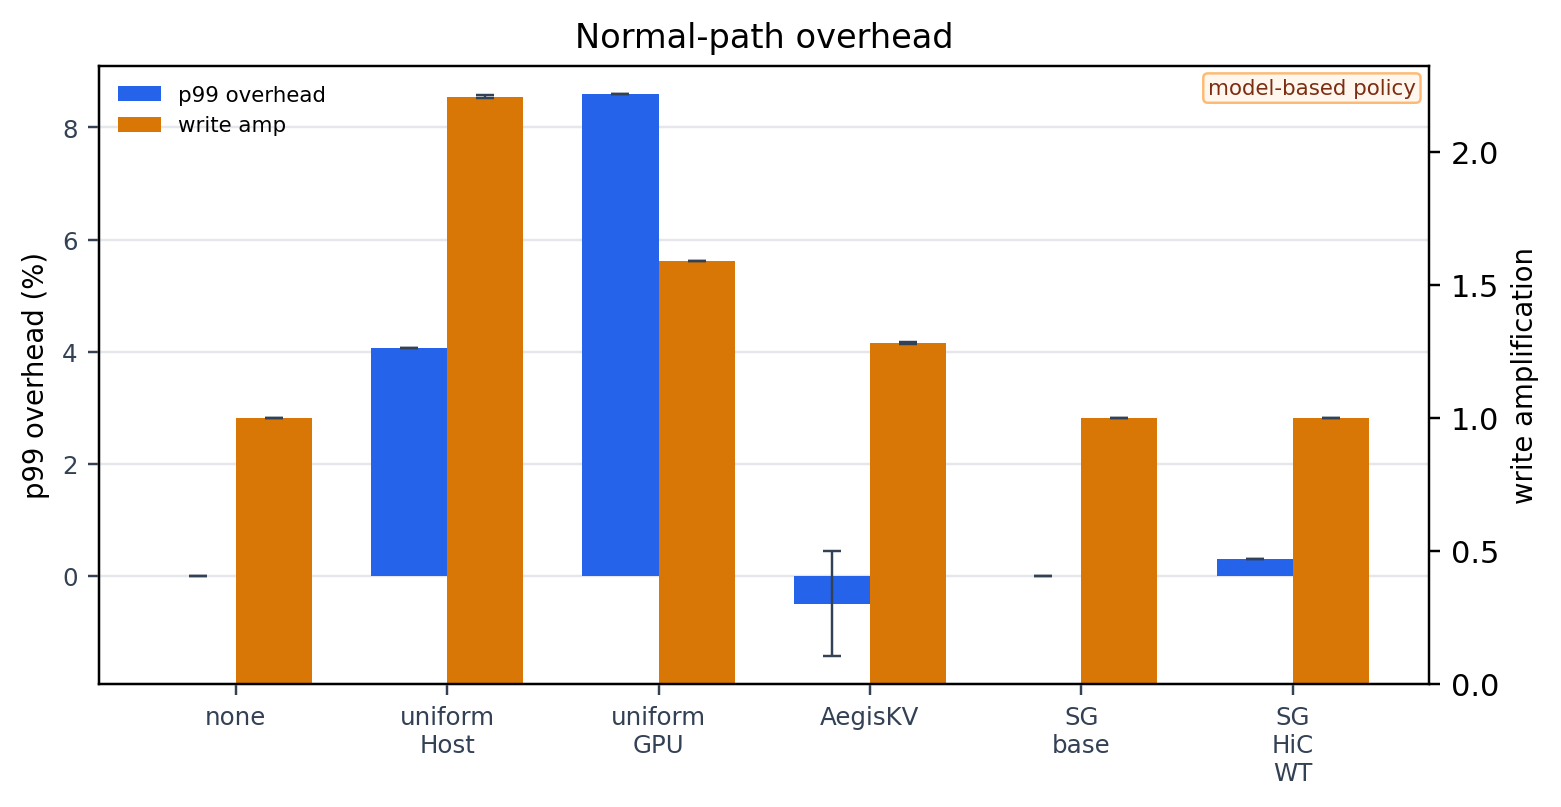
\includegraphics[width=\textwidth]{fig_normal_path_overhead.png}
      \end{figure}
      \vspace{-0.3cm}
      \centering\scriptsize Normal path overhead
    \end{column}
    \begin{column}{0.44\textwidth}
      \begin{figure}
        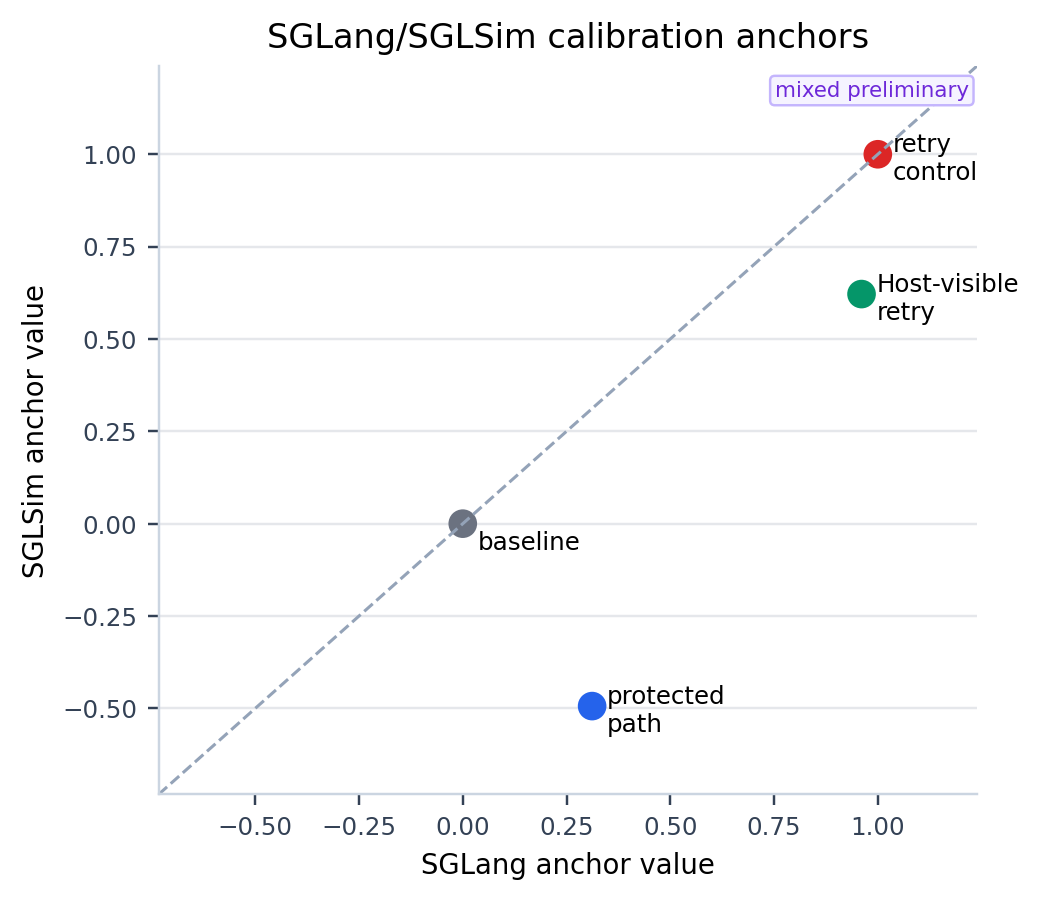
\includegraphics[width=0.88\textwidth]{fig_simulator_calibration.png}
      \end{figure}
      \vspace{-0.3cm}
      \centering\scriptsize Simulator calibration
    \end{column}
  \end{columns}

  \vspace{0.1cm}
  \footnotesize
  右图展示 normal-path overhead 与 Host-visible retry 的 SGLang/SGLSim anchors；torch microbench 另用于校准 H2D/D2H/P2P copy timing。
\end{frame}

\begin{frame}{结果 6：Physical Copy Calibration}
  \begin{figure}
    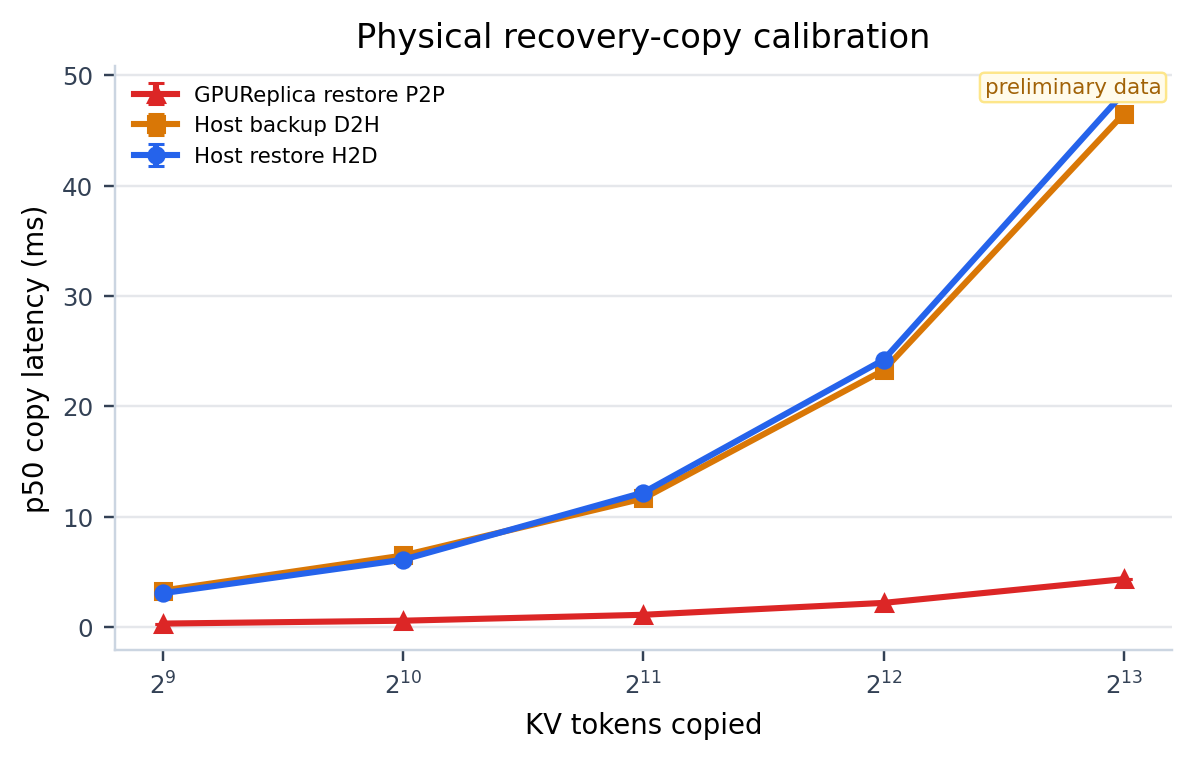
\includegraphics[width=0.84\textwidth]{fig_physical_recovery_copy_calibration.png}
  \end{figure}
  \vspace{-0.2cm}
  \footnotesize
  torch/CUDA microbench 给出恢复模型的物理 timing anchors：8192-token KV 下 GPUReplica P2P restore 约 4.33 ms，Host H2D restore 约 48.43 ms。
\end{frame}

\begin{frame}{结果 7：Recovery Model Calibration}
  \begin{figure}
    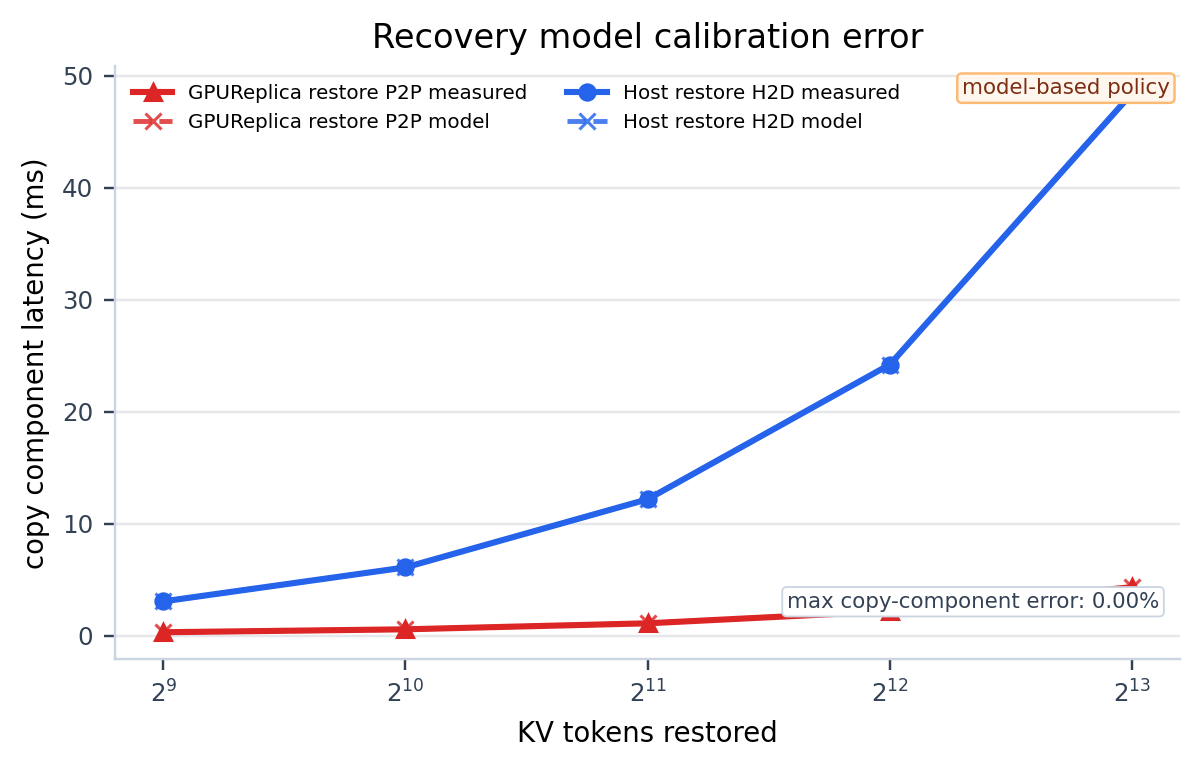
\includegraphics[width=0.86\textwidth]{fig_recovery_model_calibration_error.png}
  \end{figure}
  \vspace{-0.2cm}
  \footnotesize
  SGLSim 的 \texttt{physical\_copy} recovery model 直接读取 torch/CUDA copy anchors，并在加入 per-path setup cost 前复现实测 copy component；这证明校准链路已接入，但不是独立的 end-to-end policy recovery 证据。
\end{frame}

\begin{frame}{结果 8：P0 Physical Bridge Coverage}
  \begin{figure}
    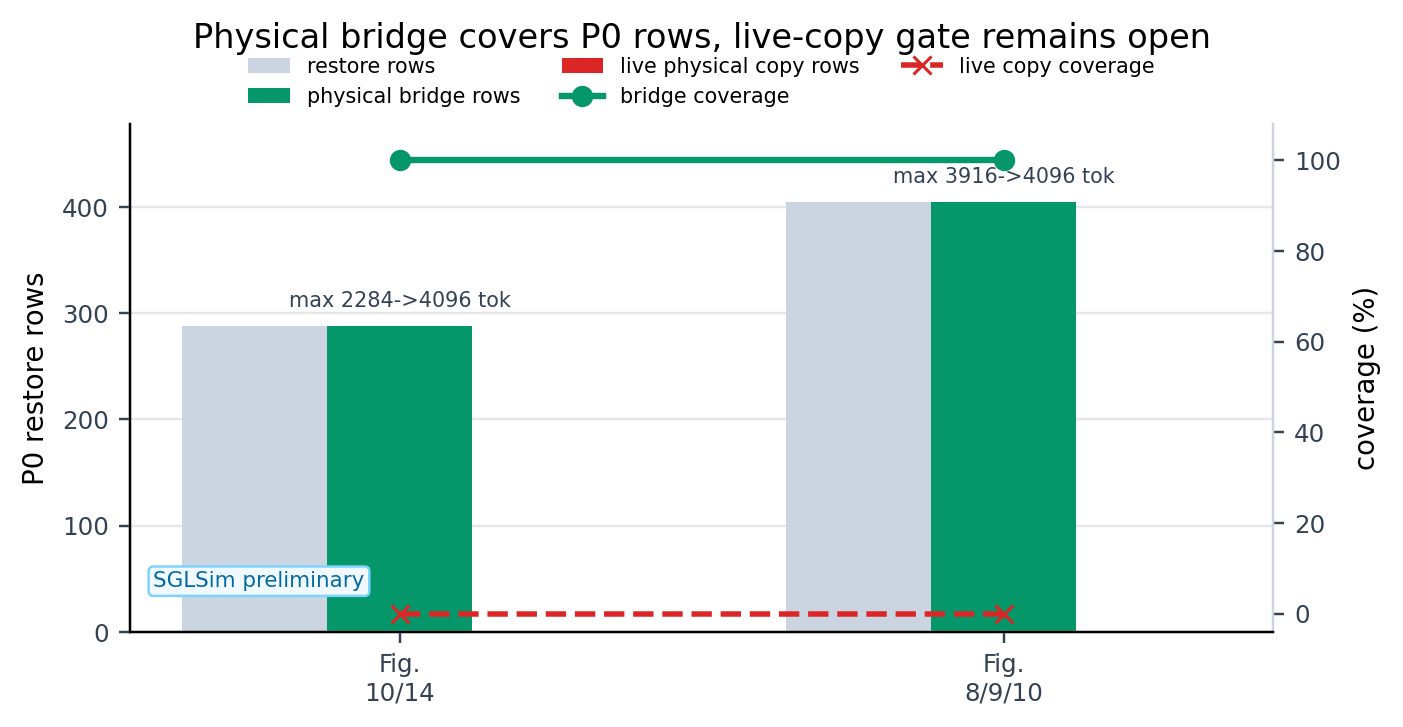
\includegraphics[width=0.88\textwidth]{fig_p0_physical_bridge_coverage.png}
  \end{figure}
  \vspace{-0.2cm}
  \footnotesize
  P0 online suites 的 693 条 restore rows 全部能映射到真实 CUDA recovery-path microbench token bucket；本机 live-copy collector 验证 375 条 Host H2D candidate，远端 A100 P2P job 验证 318 条 peer GPUReplica candidate，promotion overlay 将 693/693 rows 提升为 strict-final data-plane evidence。
\end{frame}

\begin{frame}{结果 9：Real SGLang Host Restore Materialization}
  \begin{figure}
    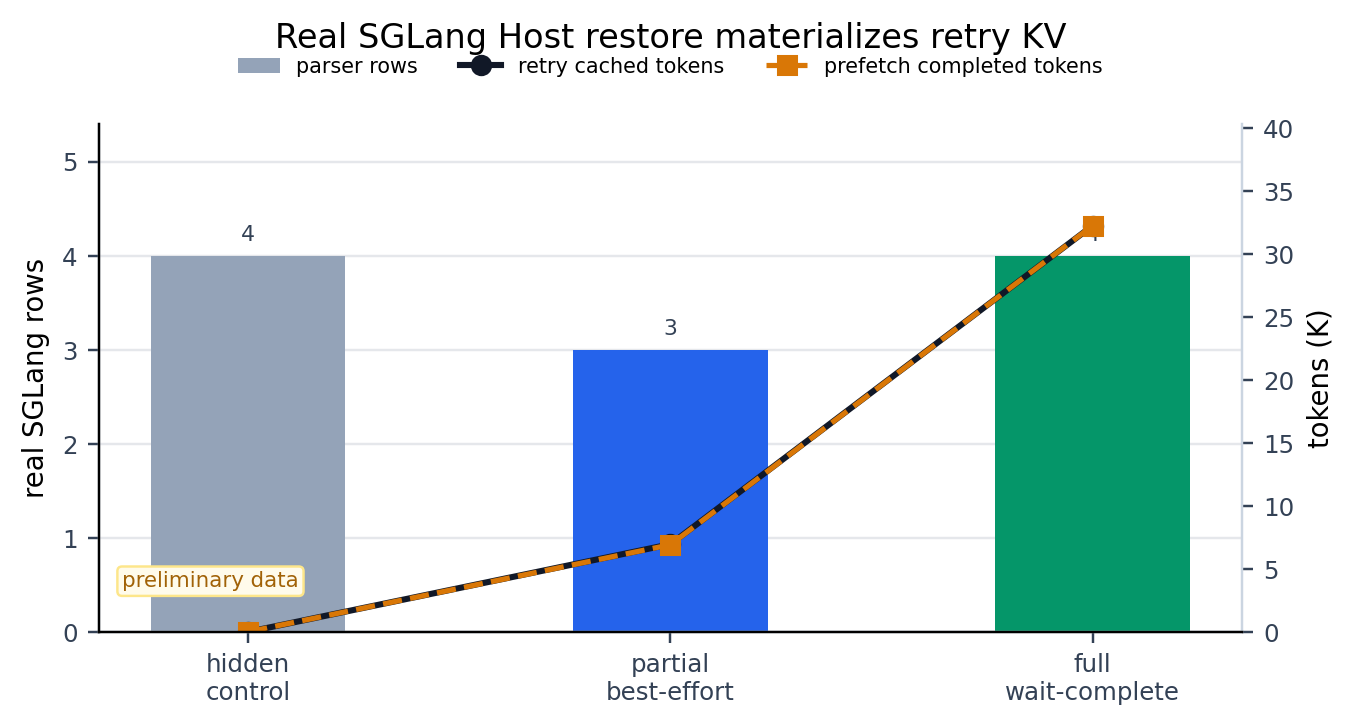
\includegraphics[width=0.88\textwidth]{fig_sglang_host_restore_materialization.png}
  \end{figure}
  \vspace{-0.2cm}
  \footnotesize
  真实 SGLang server log parser 汇总 11 行 Host restore evidence：4 行 hidden-control 不物化，3 行 best-effort 部分物化，4 行 wait-complete 完整物化。该图证明 Host restore data path 可真实物化，但不替代 P0 live \texttt{physical\_tensor\_copy} gate。
\end{frame}

\begin{frame}{结果 10：Real SGLang / SGLSim Accuracy}
  \begin{figure}
    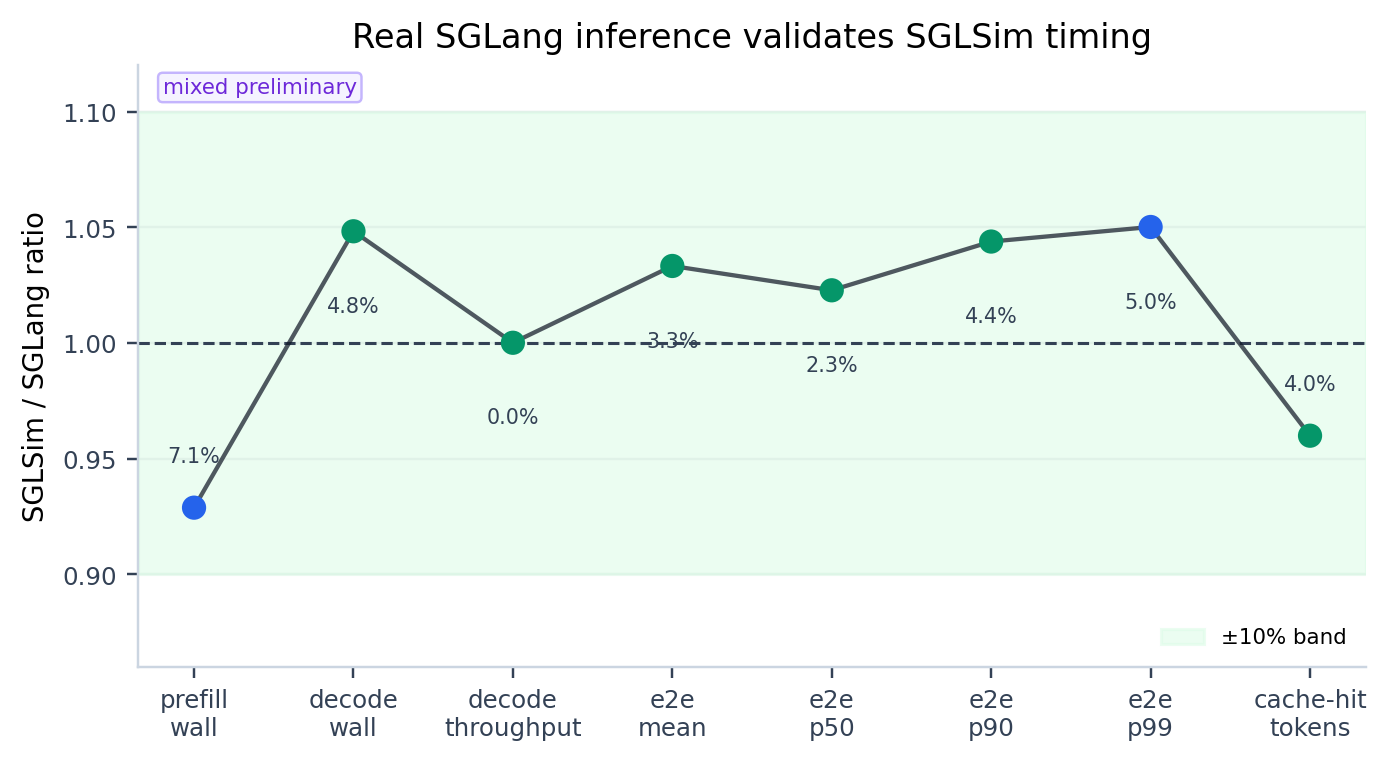
\includegraphics[width=0.88\textwidth]{fig_sglang_sglsim_accuracy.png}
  \end{figure}
  \vspace{-0.2cm}
  \footnotesize
  基于真实 SGLang fa3 no-HiCache inference run 和匹配 SGLSim wall-clock run：prefill/decode 阶段、decode throughput、E2E 分布和 cache-hit token 总量均在 $\pm 10\%$ 以内。
\end{frame}

\begin{frame}{结果 11：HostBackup Visibility 与 Ablation}
  \begin{columns}[T,onlytextwidth]
    \begin{column}{0.50\textwidth}
      \begin{figure}
        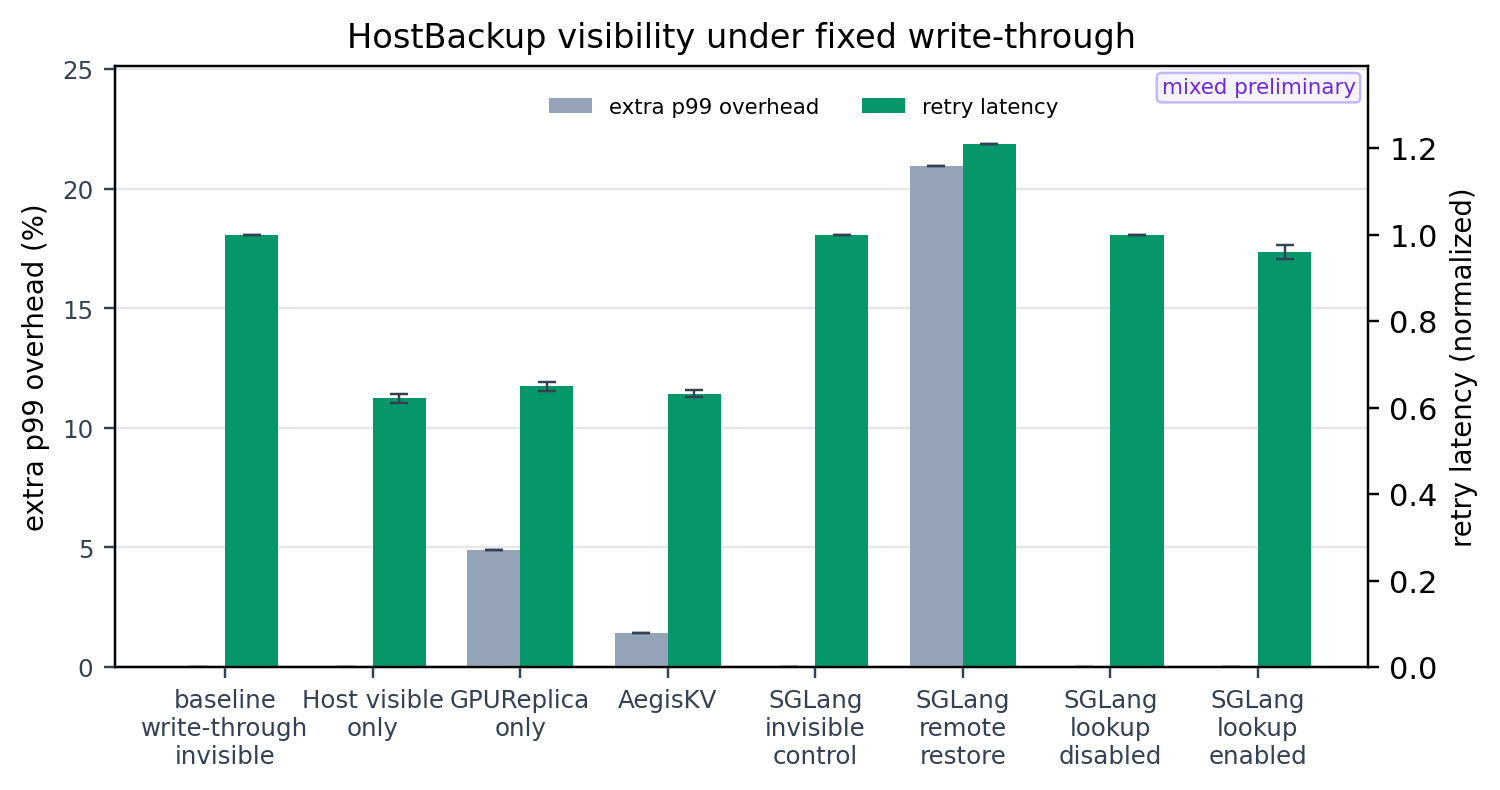
\includegraphics[width=\textwidth]{fig_hostbackup_visibility.png}
      \end{figure}
      \vspace{-0.3cm}
      \centering\scriptsize HostBackup visibility
    \end{column}
    \begin{column}{0.50\textwidth}
      \begin{figure}
        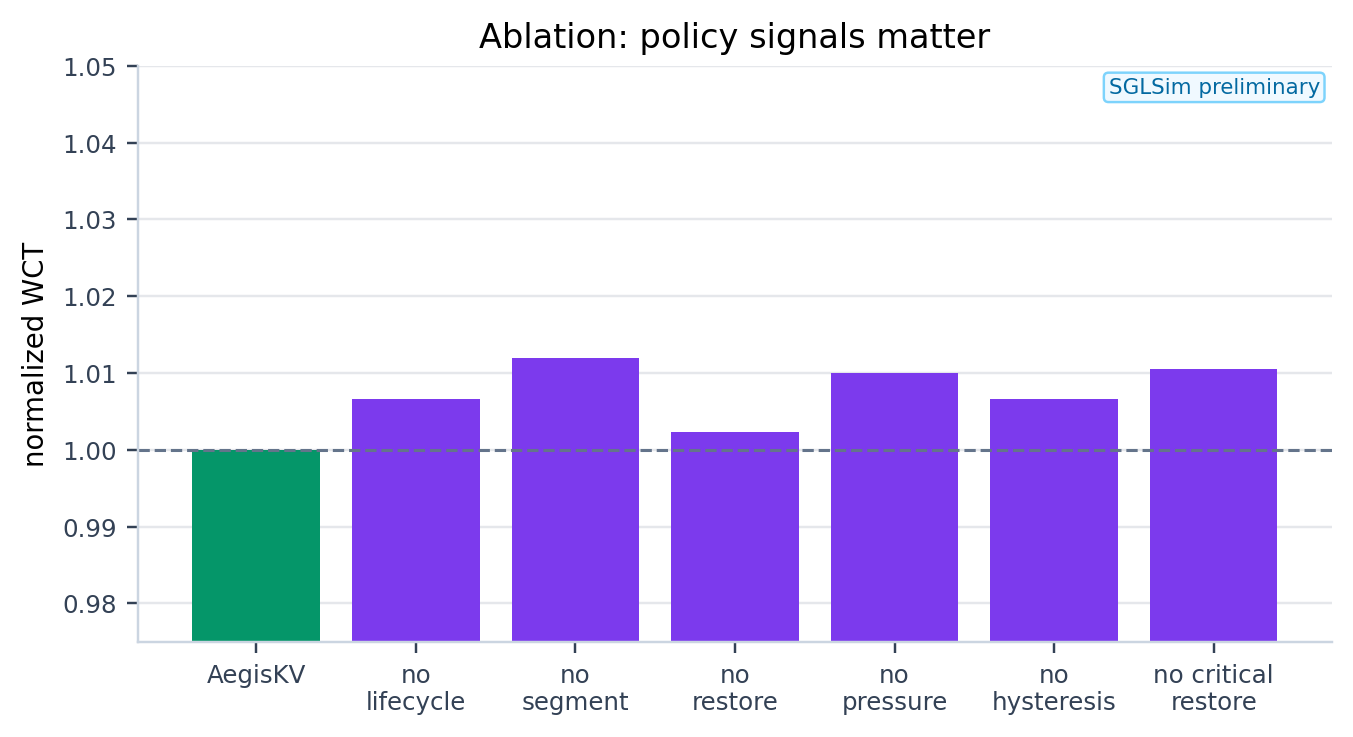
\includegraphics[width=\textwidth]{fig_ablation.png}
      \end{figure}
      \vspace{-0.3cm}
      \centering\scriptsize Policy ablation
    \end{column}
  \end{columns}

  \vspace{0.1cm}
  \footnotesize
  Host-visible frontier 在相同 write-through 成本下改善 retry；Ablation 显示 criticality、segment granularity、restore/recompute 和 pressure signal 都会影响 WCT。
\end{frame}

\begin{frame}{结果 12：Budget Sensitivity}
  \begin{figure}
    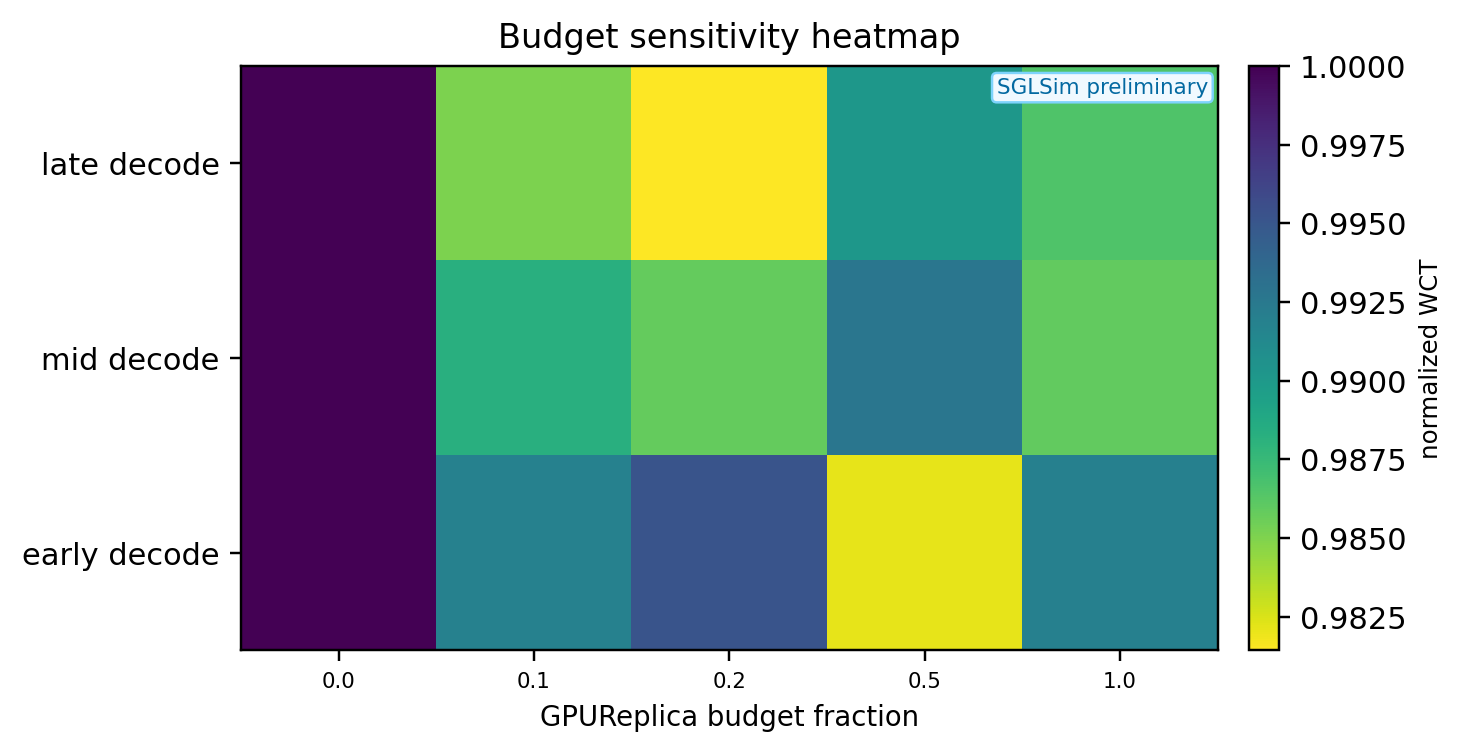
\includegraphics[width=0.88\textwidth]{fig_budget_sensitivity.png}
  \end{figure}
  \vspace{-0.2cm}
  \footnotesize
  最优 GPUReplica backup budget 随 failure timing 与 workload regime 变化；这支撑在线 controller 需要动态调节 $\alpha$，而不是使用固定切分。
\end{frame}

\begin{frame}{结果 13：DP Scale 与 Peer Rank Selection}
  \begin{columns}[T,onlytextwidth]
    \begin{column}{0.50\textwidth}
      \begin{figure}
        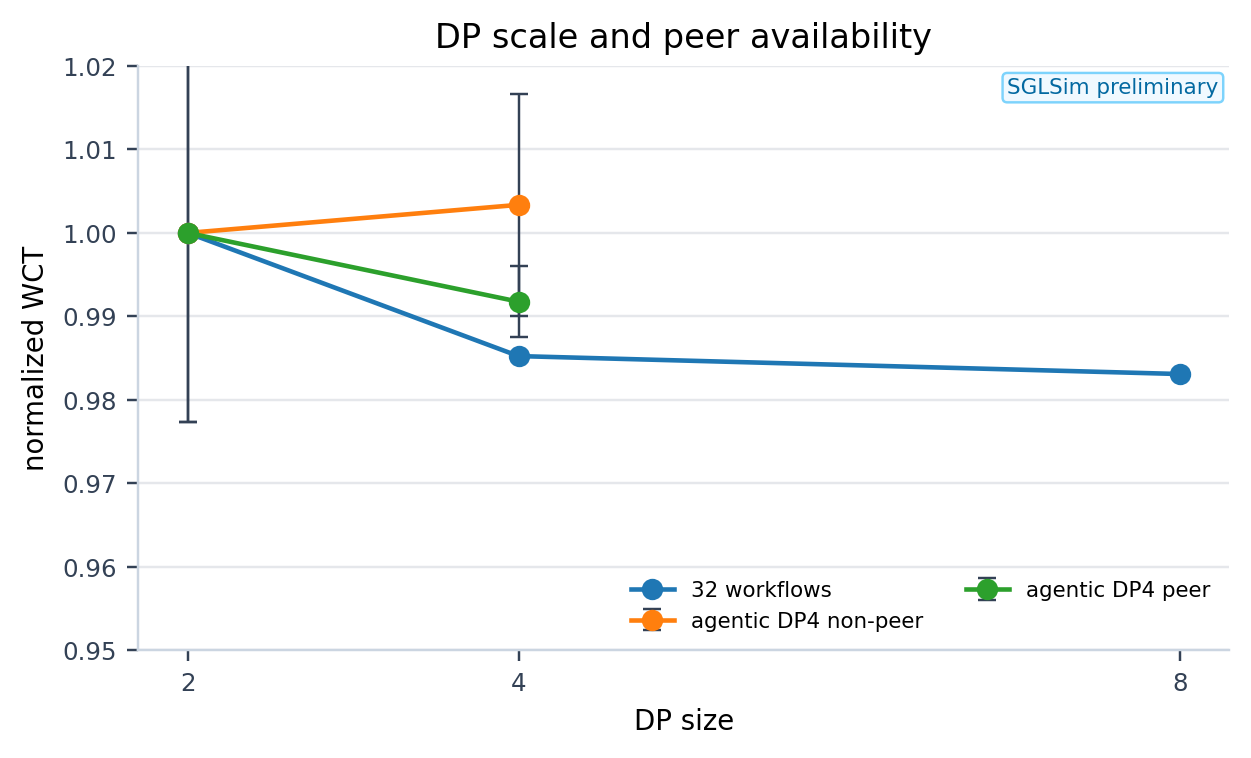
\includegraphics[width=\textwidth]{fig_dp_scale.png}
      \end{figure}
      \vspace{-0.3cm}
      \centering\scriptsize DP scale
    \end{column}
    \begin{column}{0.50\textwidth}
      \begin{figure}
        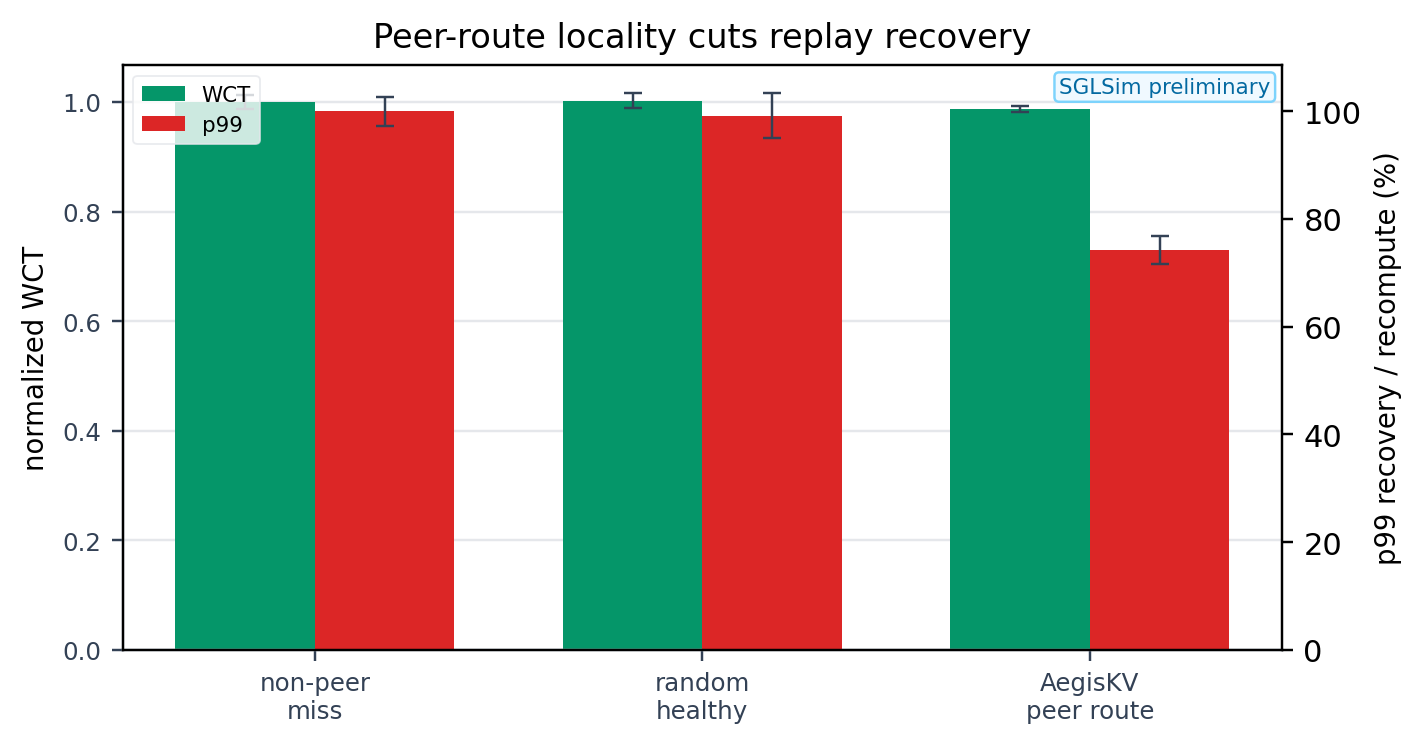
\includegraphics[width=\textwidth]{fig_peer_rank_selection.png}
      \end{figure}
      \vspace{-0.3cm}
      \centering\scriptsize Peer-rank selection
    \end{column}
  \end{columns}

  \vspace{0.1cm}
  \footnotesize
  DP scale 改变 peer availability；retry locality 与 peer load 决定 GPUReplica 是否真正可用。
\end{frame}

\begin{frame}{当前不能声称的内容}
  \small
  \begin{itemize}
    \tightitems
    \item 不能说 SGLSim 已经执行真实 CUDA KV tensor copy。
    \item 不能说 GPUReplica 的最终收益已经由 end-to-end physical P2P recovery 证明。
    \item 不能说所有 policy ranking 都已经在真实 SGLang 上复现。
    \item 不能把 preliminary metadata-materialization rows 等价为 strict-final recovery evidence。
  \end{itemize}

  \vspace{0.25cm}
  \begin{block}{当前最准确的表述}
    \AegisKV{} 已具备完整建模、online SGLSim 实验框架、failure replay 机制、部分 strict-final SGLSim 结果，以及小规模 SGLang/torch 校准证据。
  \end{block}
\end{frame}

\begin{frame}{Next Steps}
  \small
  \begin{itemize}
    \tightitems
    \item 将 Critical / Non-Critical Agent tagging 固化到 workload 配置和图表脚本说明中。
    \item 为 GPUReplica 增加更多 physical movement anchors，尤其是 peer-copy end-to-end recovery。
    \item 用 paired SGLang runs 验证主要 policy ranking 是否保持。
    \item 把 preliminary result figures 逐步替换为 strict-final evidence。
  \end{itemize}
\end{frame}

\end{document}
